\documentclass[12pt]{article}
\usepackage{fullpage}
\usepackage[noend]{algpseudocode}
\usepackage{algorithmicx}
\usepackage{algorithm}
\usepackage{amssymb}
\usepackage{amsmath}
\usepackage{graphicx}
\usepackage[bottom]{footmisc}
\newcommand{\realpositivenumbers}{\mathbb{R}_{>0}} %Real numbers symbol
\newcommand{\bigO}{\mathcal{O}}

\begin{document}

\section*{ADM (2019) - Homework 2}

\subsection*{Theoretical Question}
\vspace{.5cm}

You are given the following functions:
\vspace{.4cm}


\begin{algorithm}
\caption{splitSwap}\label{splitFun}
\begin{algorithmic}[1]
\Function{splitSwap}{a, i, n}:
\If {$i \leq 1$} 
	\State \Return 
\EndIf

\State \Call{splitSwap}{a, $i$, $n/2$}
\State \Call{splitSwap}{a, $i+n/2$, $n/2$}
\State \Call{swapSplit}{a, $i$, $n$}
\EndFunction
\end{algorithmic}
\end{algorithm}

\begin{algorithm}
\caption{swapList}\label{swapFun}
\begin{algorithmic}[1]
\Function{swapList}{a, l, n}:
\For {$i=0 \leq n/2$}
\State tmp = a[$l + i$]
\State a[$l + i$] = a[$l + i + n/2$]
\State a[$l + i + n/2$] = tmp
\EndFor
\EndFunction
\end{algorithmic}
\end{algorithm}

\begin{enumerate}
\item How much running time does it take to execute \textproc{splitSwap}(a, 0, n)? Use Big-O analysis.
\item What does this algorithm do? Is it optimal? Describe the mechanism of the algorithm in details, we do not want to know only its final result.
\end{enumerate}
\pagebreak

\section*{Solution}

\subsection*{Question 1}

Let's start by first analyzing the second function, \textproc{swapList} as it is called inside the other function we want to 
analyze. 

We can split the code into two parts: the assignments (which allow us to swap two values) and the loop.
Then we can start writing the analysis for time complexity of this function: 

$$ T_2(n) = 3\ c_1 \cdot (c_2\ (n/2))$$

This means that we suppose each of the 3 assignment to take approximately $c_1$ units of time. The loop performs a check for
each iteration, hence $c_2$.
We can already start dropping lower order terms and constants that don't help us with the analysis, so we have that:
$$ T_2(n) = n/2 $$

We can now try to find a function that allow us to define the complexity of the \textproc{splitSwap} function.
\vspace{1cm}

Let $f(n) = n $ and $g(x) = T_2(n) = n/2$. If we are able to find a $c \in \realpositivenumbers$ such that for 
any $n \geq n_0$ we have that $g(n) \leq cf(n)$, we can say that \textproc{splitSwap} is $\bigO(n)$.

We have:

$$ \frac{n}{2} \leq c\ n $$
$$ 1 \leq 2c $$
$$ c \geq \frac{1}{2} $$

Let's try to find a lower bound for our function in analysis. We choose $h(n) = n$ and $g(n) = n / 2$, and see if we find a $c \in \realpositivenumbers $ such that for each $n \geq n_0$ we have that $g(n) \geq c\ h(n)$.

$$ g(n) \geq c f(n) $$
$$ n/2 \geq c n $$
$$ c \leq \frac{1}{2} $$

We have found a constant so that $g(x) \geq \frac{1}{2}\ f(x)$ for all $n \geq n_0$, so we can say that $g(x)$ is $\Omega(n)$.
\vspace{1cm}

Since we want also to build a tighter bound for defining the complexity of $g(x)$, we can intersect the previously found sets of constants $c$ such that $c\ f(n) \geq g(n) \geq c\ h(n)$, we find that $c = \frac{1}{2}$ is the only solution.

Having found such constant, we can now say that $g(n)$ is $\theta (n)$.
\pagebreak

We can now start analyzing the complexity of \textproc{splitSwap}. Since we found that \\ \textproc{swapList} is $\theta(n)$ we 
can put it easily in the \textproc{splitSwap} recursive definition:

\begin{equation}
  T(n) =\begin{cases}
    \theta(1) & \text{if $n \leq 1$}.\\
    2T\left( \frac{n}{2} \right) + \theta(n) & \text{otherwise}
  \end{cases}
\end{equation}

The algorithm is in a \textit{divide-et-impera} recurrence form and the way such recurrence is defined might 
allow the use of the Master Theorem. Let's first see how the recurrence relation in the MT presents itself in variable form: 

\begin{equation}
	T(n) = a T\left( \frac{n}{b} \right) + f(n)
\end{equation}

Choosing $a = 2$, $b = 2$, and $f(n) = n$ we get:

\begin{equation}
	T(n) = 2 T\left( \frac{n}{2} \right) + n
\end{equation}

Which is the inductive case definition of \textproc{splitSwap} (so for $n > 1$). This algorithm is shown to be 
$\theta(n \log{n})$, in the case of $f(n) = \theta(n^{log_b{a}}) = \theta(n^{log_2{2}}) = \theta(n)$ and assuming that $n$ is 
a perfect power of $2$.
                                                                                                                                                                                                                                                                     

                                                                                                                                                                                                                                                                    It might be easier to visualize using this recursion tree representation:
                                                                                                                                                                                                                                                                    \begin{figure}[h]                                                                                                                                                                                                                                                                    \caption{Image from \textit{Introduction to Algorithms, CLRS}}                                                                                                                                                                                                                                                                     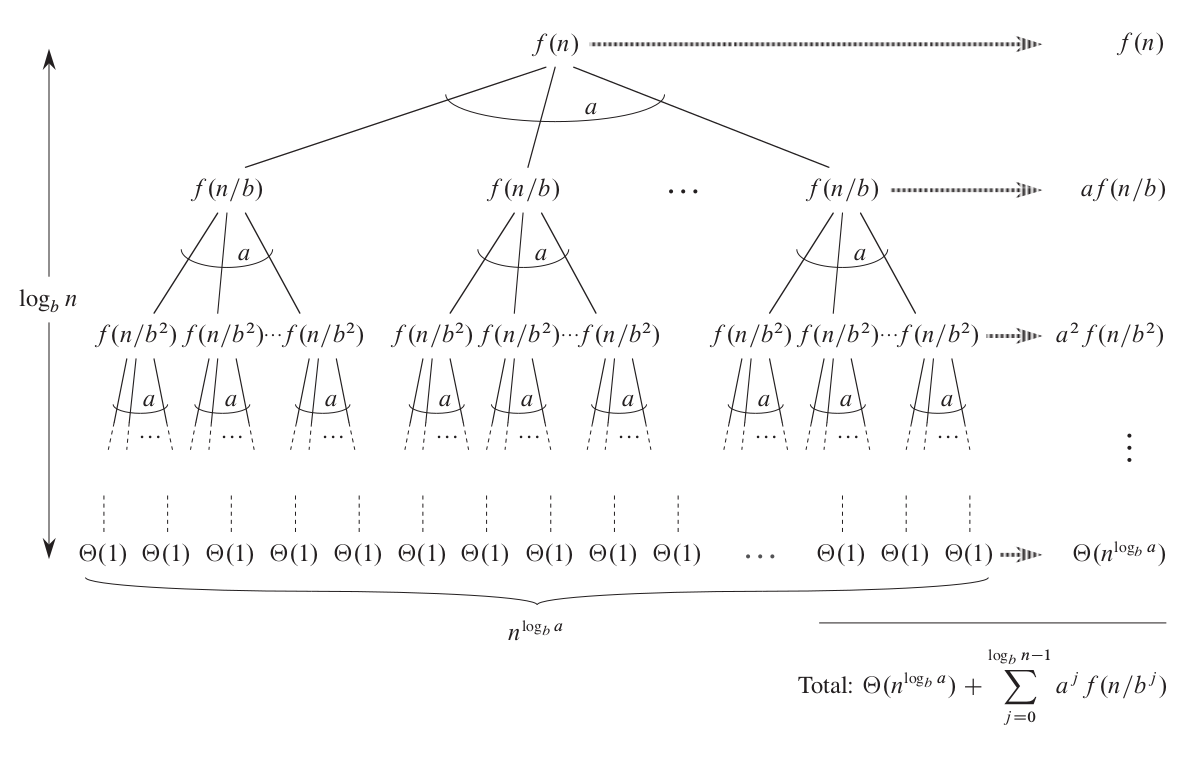
\includegraphics[scale=.35]{./recursion_tree_clrs.png}                                                                                                                                                                                                                                                                   
\centering
\end{figure}

We can see that for each splitting of the array the function is being called $log_2{(n)}$ times, each call will cost us $\theta(n)$, hence our result $\theta(n\ log_2{(n)}$.

\subsection*{Question 2}

The algorithm in analysis, according to what we found, is supposed to reverse a list of integers, where the number of the elements
list should be $2^n$: this is the ideal case. Unfortunately if the list size differs from a number expressed as $2^n$, it behaves
differently. 
\vspace{.4cm}

For example, if we consider an array of size $2^k + 1$, we found the list is correctly reversed except for the last element, which
is left where it originally was. For a size of $2^k + 2$ the list is reversed,except for at position $(2^k + 2)/2$ and the last element, which are swapped.
\vspace{.4cm}

Such behaviour is caused by the nature of the definition of the recursive step $2T(n/2)$, which might not be effective 
when $n$ is not a power of $2$. It brings rounding errors in the indexes used for splitting the array and swapping elements.

\subsubsection*{What does it do?}

For $n > 1$, the \textproc{splitSwap} function splits\footnotemark[1]   the array into two halves. It continues to do so for each sub-array, 
until a minimum sub-array size is reached. It then starts merging\footnotemark[1] using \textproc{swapList} the two sub arrays at a time,
swapping the order of the elements from left to right: this means that the element at index $i$ is swapped with the one at 
$i + n'/2$, then $i$ is incremented by $1$. Side note, $n'$ is the size of the sub-array and $i$ is incremented until it reaches
the value of $n'/2$

From line 4 of \textproc{splitSwap} we can observe that the split-merge-reverse happens to the first half of the array first, 
then the second one, until both halves are ready to be merged again (before one last swapping across them). 

\subsubsection*{Is it optimal?}

In the ideal case, so when the size of the array is a power of 2, then no: for three reasons. First the number of steps could 
be significantly reduced. Given an array of length $n$, doing the swapping on the elements at index $i$ and $(n-i)$ then incrementing $i$ until reaching the value $i = n/2$, brings better performance (it is executed in linear time). 

The second reason is memory allocated for the array in the ideal case: having $2^k$ elements in memory becomes a problem for 
high values of $k$. The third reason is a consequence of the previous point: the number of recursive calls might be ignored since it is the logarithm of the size of the array, but doing the swapping for $2^k$ elements might be problematic for high values of $k$ (tests showed this).
\vspace{.4cm}

In the non-ideal case, where the size of the array is not expressed as a power of 2, it's hard to tell if it's optimal. For such an array the algorithm does not reverse the list, since some elements end up at the wrong index (when compared to the 
expected result of an array reversing algorithm). 	

\footnotetext[1]{When talking about splitting and merging we don't mean that this happens by using multiple separated references for each sub-array. We mean that the indexes allow us to consider only portions of the array.}
\end{document}
